\documentclass[a4paper, 12pt, titlepage]{article}

% Document quality things
\usepackage[utf8]{inputenc}
\usepackage{microtype, xcolor}
\usepackage{csquotes}
\usepackage{url, hyperref}
\hypersetup{colorlinks=true, linkcolor=black, citecolor=black, urlcolor=blue}

% Image-related packages
\usepackage{graphicx}
%\usepackage{float}
\graphicspath{{./gfx/}}
%\usepackage[font=small,skip=5pt]{caption}

% Setting margins
\usepackage[a4paper,bottom=2cm,top=2cm,left=2.5cm,right=2.5cm, includefoot]{geometry}

% Table helper packages
%\usepackage{multirow, multicol}
%\usepackage{makecell}
%\usepackage{array}
%\usepackage{tabularx} % Not needed currently, but has a few nice options
%\usepackage{wrapfig} % Floating figures/tables
\usepackage{booktabs}
\usepackage{longtable}

% Prevents spamming tedious newlines everywhere, also disables auto indentation, etc.
\usepackage[skip=0.75\baselineskip plus 2pt]{parskip}

% Self-explanatory
%\usepackage{titlesec}
%\titleformat{\section}[block]{\normalfont\scshape\Large}{\thesection}{1em}{}
%\titleformat{\subsection}{\normalfont\large}{\thesubsection}{1em}{}

\title{
    {CS 319 - Object Oriented Software Engineering}\\
    {\small Instructor: Eray Tüzün, TA: Muhammad Umair Ahmed}\\
    {\vspace{10mm}BilHealth}\\
    {\Large \textbf{Analysis Report}}\\
    {\small Iteration 1}\\
    {\vspace{10mm}
\includegraphics[width=0.3\linewidth]{bilkentlogo}}
}
\author{
  Mehmet Alper Çetin\\ \texttt{21902324}
  \and
  Vedat Eren Arıcan\\ \texttt{22002643}
  \and
  Uygar Onat Erol\\ \texttt{21901908}
  \and
  Recep Uysal\\ \texttt{21803637}
  \and
  Efe Erkan\\ \texttt{21902248}
}
\date{\today}

% \usepackage{tikz}
% \usetikzlibrary{automata, positioning, arrows}

\usepackage{pdflscape, pdfpages}

\begin{document}
  \maketitle
  \tableofcontents
  \pagebreak

  \section{Introduction}

  Our project is a health center management software, built in the form a web application.
  The main goal is to provide online, remote attention to patients to increase productivity for all parties involved.
  The primary method of interaction is through \textit{case}s, which contain all relevant information for a given medical situation.
  Patients use the system to open cases and request appointments, and the health center staff acts on these requests
  to provide medical services.

  Note that all diagrams on this document are in vector format, meaning that you can zoom in without any decrease in quality.

  \section{Current System}

  Our team has visited the Bilkent University health center to inquire about the application domain,
  along with the existing system they have in place.
  Our initial assumptions were then altered to respect their practical requirements.

  The people interviewed were a staff member of the secretary,
  the head nurse, and the director of the health center.
  Consequently, below is a concise list of our findings.

  \begin{itemize}
    \item New patients are first examined by a nurse, after which the patient may be triaged to a medical specialist.
    \item During triaging, the nurse may measure the patient's heart rate, body temperature, blood pressure, etc.
      These details are naturally provided to the specialist who provides medical care to the patient.
    \item Triaging is not necessary for patients whose concerns fall into the psychological and dental domains.
    \item Appointments by phone are not available to students, as many do not show up to their appointments.
    \item Anyone who enters the health center for an examination has their records created in the system.
    \item Their system is in no way connected to the state's health system, named \textit{E-Nabız}.
    \item Medical test results are stored in the system. The system is directly integrated with the devices carrying out the tests.
    \item The planning of the materials, budget, and such, takes into account the data stored in their patient record system.
    \item Personal medical records are kept in detail, including vaccination cards.
    \item Personal medical records are visible solely to the medical staff member who is responsible for the patient.
    \item The primary patient base is comprised of students.
      Those who stay in the university's housing, or are a part of the university personnel, are secondary.
      Needless to say, health care is given to anyone in a moment of emergency.
    \item As opposed to a patient's personal medical records,
      the medical staff is able to share notes about a particular visit,
      viewable by other medical staff.
    \item Patients reserve the right to choose their own caregivers.
      In any other case, the nurse is responsible for the triaging.
  \end{itemize}

  \section{Proposed System}

  Our design was created with the context of Bilkent University in mind, as made clear by the project name.
  Some of our assumptions include the system maintained by the Bilkent Computer Center (BCC).
  For instance, we have assumed that majority of the patient base could be created through the general student records
  kept by the institute, and as such have forgone a public registration endpoint.

  \subsection{Actors}

  Health system management is a complex domain with many actors involved.
  Based on the current systems used, we have created five actor types to interact with the system in various capacities.

  \begin{itemize}
    \item \textbf{Nurse:} Part of the medical staff that can record patient data and forward patients to doctors.
    \item \textbf{Doctor:} Part of the medical staff that can undertake cases opened by patients.
    \item \textbf{Staff:} Part of the health center staff, but not for medical tasks, and as such cannot accept cases.
      They are mostly able to perform a subset of doctor and patient features on their behalf, so as to manage the process.
    \item \textbf{Patient:} Able to open cases and receive medical attention as a result of their interaction with the system.
    \item \textbf{Admin:} Manages the system but is not necessarily a part of the health center staff.
      This is a role for developers/maintainers of the system to do housekeeping, such as mass registering new users.
  \end{itemize}

  \pagebreak
  \subsection{Functional Requirements}

  We have split up our functional requirements into actor types, to ease interpretation.

  \textbf{Nurse:}
  \begin{itemize}
    \item A nurse, upon the initial visit to an open case, should be able to request a forward/triage to a specific doctor
    \item A nurse should be able to record patient details during the visit, such as heart rate, blood pressure, and body temperature
    \item A nurse should be able to update patient profile details
  \end{itemize}

  \textbf{Doctor:}
  \begin{itemize}
    \item A doctor should be able to receive open cases and provide medical attention online then on premise through appointments
    \item A doctor should be able to close cases when there is no longer a medical situation needing attention
    \item A doctor should be able to record notes about a patient's visit, viewable by other doctors
    \item A doctor should be able to follow up online on patients through the cases they have opened
    \item A doctor should have a profile with relevant information such as area of medical expertise
    \item A doctor should be able to add prescriptions to cases and generate printable documents for pharmacies
    \item A doctor should be able to approve appointment requests in cases, or cancel approved appointments
    \item A doctor should be able to make site-wide announcements
    \item A doctor should be able to request an inclusive anonymous report of campus-wide patient data
  \end{itemize}

  \textbf{Staff:}
  \begin{itemize}
    \item A staff member should be able to view cases, but without the ability to provide any medical assistance
    \item A staff member should be able to open cases on behalf of patients, and close them when necessary
    \item A staff member should be able to approve triaging requests made by nurses
    \item A staff member should be able to update patient profile details
    \item A staff member should be able to upload test result PDFs onto the system
    \item A staff member should be able to make site-wide announcements
    \item A staff member should be able to request an inclusive anonymous report of campus-wide patient data
  \end{itemize}

  \textbf{Patient:}
  \begin{itemize}
    \item A patient should be able to open a case to seek medical attention by specifying concerns
    \item A patient should be able to request appointments through the case they've opened
    \item A patient should be blacklisted from requesting an online appointment, if they repeatedly do not show up to their appointments
    \item Each appointment should contain a visit that holds information such as heart rate, body temperature, blood pressure, etc.
    \item A patient should be able to follow up with cases by adding messages onto the open case
    \item A patient should have a medical profile with medical history and relevant information such as past cases, physical measurements, vaccination history, etc.
    \item A patient should automatically have their medical profile made visible to the medical staff member responsible for their case
    \item A patient should be able to view their medical test results online
    \item A patient should be able to view announcements made by the health center
    \item A patient should receive notifications about updates to their cases, through the website or email
    \item A patient should be able to request a machine-generated report of personal medical history
    \item A patient should be able to use the service to do basic medical calculations such as BMI measurements
  \end{itemize}

  \textbf{Admin:}
  \begin{itemize}
    \item An admin should be able to register new users, including mass registering them
    \item An admin should be able to monitor the system by having access to most parts of the system views
  \end{itemize}

  \pagebreak
  \subsection{Non-functional Requirements}

  Our non-functional requirements are as follows:

  \begin{itemize}
    \item \textbf{Security:} Since a person's health details are highly privacy sensitive, the system should protect a patient's records from any unauthorized activity
    %\item \textbf{Usability:} The system and its user interface should be easily usable by all actors in order to achieve its goal of increasing productivity
    \item \textbf{Usability:} The system should be easy to learn by making the user interface easy to understand
    \item \textbf{Reliability:} The users' expectation of the system to be predictable in its reactions to user interaction should be satisfied
    \item \textbf{Scalability:} The system should be able to comfortably support a user base of up to 20000 users, with leeway for more
    \item \textbf{Maintainability:} The system should be implemented in a way that is practical to maintain
    \item \textbf{Deployment:} The system should not be tightly coupled with its hosting environment, to be able to deploy on most servers with ease
    \item \textbf{Extensibility:} The system should be implemented in a way that allows developers to extend functionality without refactoring majorly
    \item \textbf{Fault tolerance:} The system should be able to run despite database connection errors, and notify maintainers and users when a problem occurs
    \item \textbf{Integrability:} The system should be able to integrate services from another software system, such as Bilkent University's BCC infrastructure
    \item \textbf{Testability:} The system should be implemented in a way that allows automated testing tools to be used
  \end{itemize}

  \subsection{Pseudo Requirements}

  \begin{itemize}
    % \item The system on the server side should be implemented in C\#, using the ASP.NET Core library
    % \item The user interface should be implemented in TypeScript, using React.js
    % \item The system should use PostgreSQL as its data persistence solution
    \item The system should be implemented by using Object-Oriented Programming principles
    \item The system should be implemented as a web application
  \end{itemize}

  \pagebreak
  \subsection{Scenarios}

  The average user experience on the project should be similar to the following scenario.

  \begin{enumerate}
    \item The patient logs into the system with their institute-provided credentials
    \item The patient opens a case and specifies their concerns
    \item The patient schedules their first appointment
    \item The patient visits the health center at the time of the appointment
    \begin{itemize}
      \item A nurse performs an initial examination, and if necessary, requests to forward the case to a specialist
      \item The triage request may be approved by a staff member
    \end{itemize}
    \item A doctor is assigned to the case as a result of triaging
    \item The patient schedules another appointment \textit{(Repeat from step 4)}
  \end{enumerate}

  \pagebreak
  \subsection{System Models}

  \subsubsection{Use Case Diagram}

  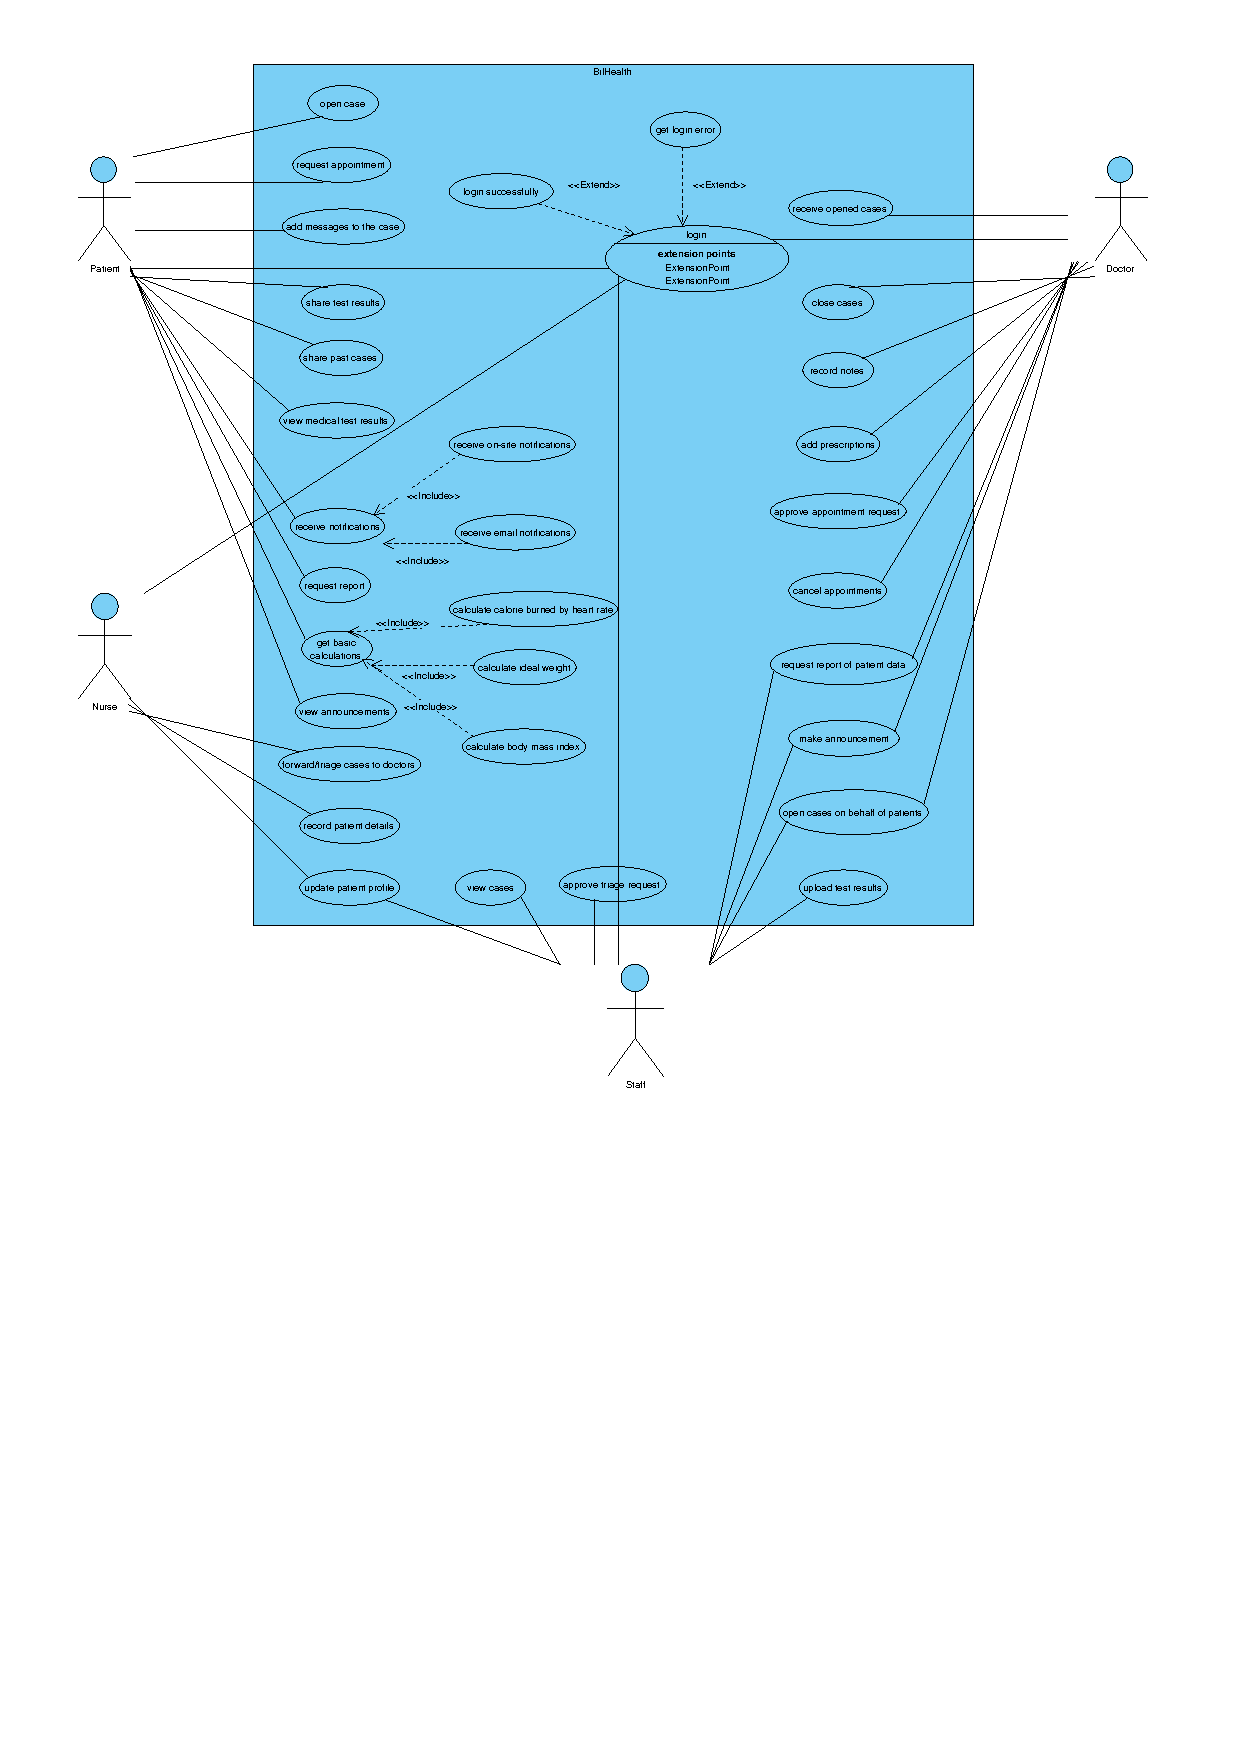
\includegraphics[width=\linewidth]{use_case_diag}

  \pagebreak
  \subsubsection{Activity Diagram}

  The following diagram shows the general flow of activities as a patient attempts to get an appointment.

  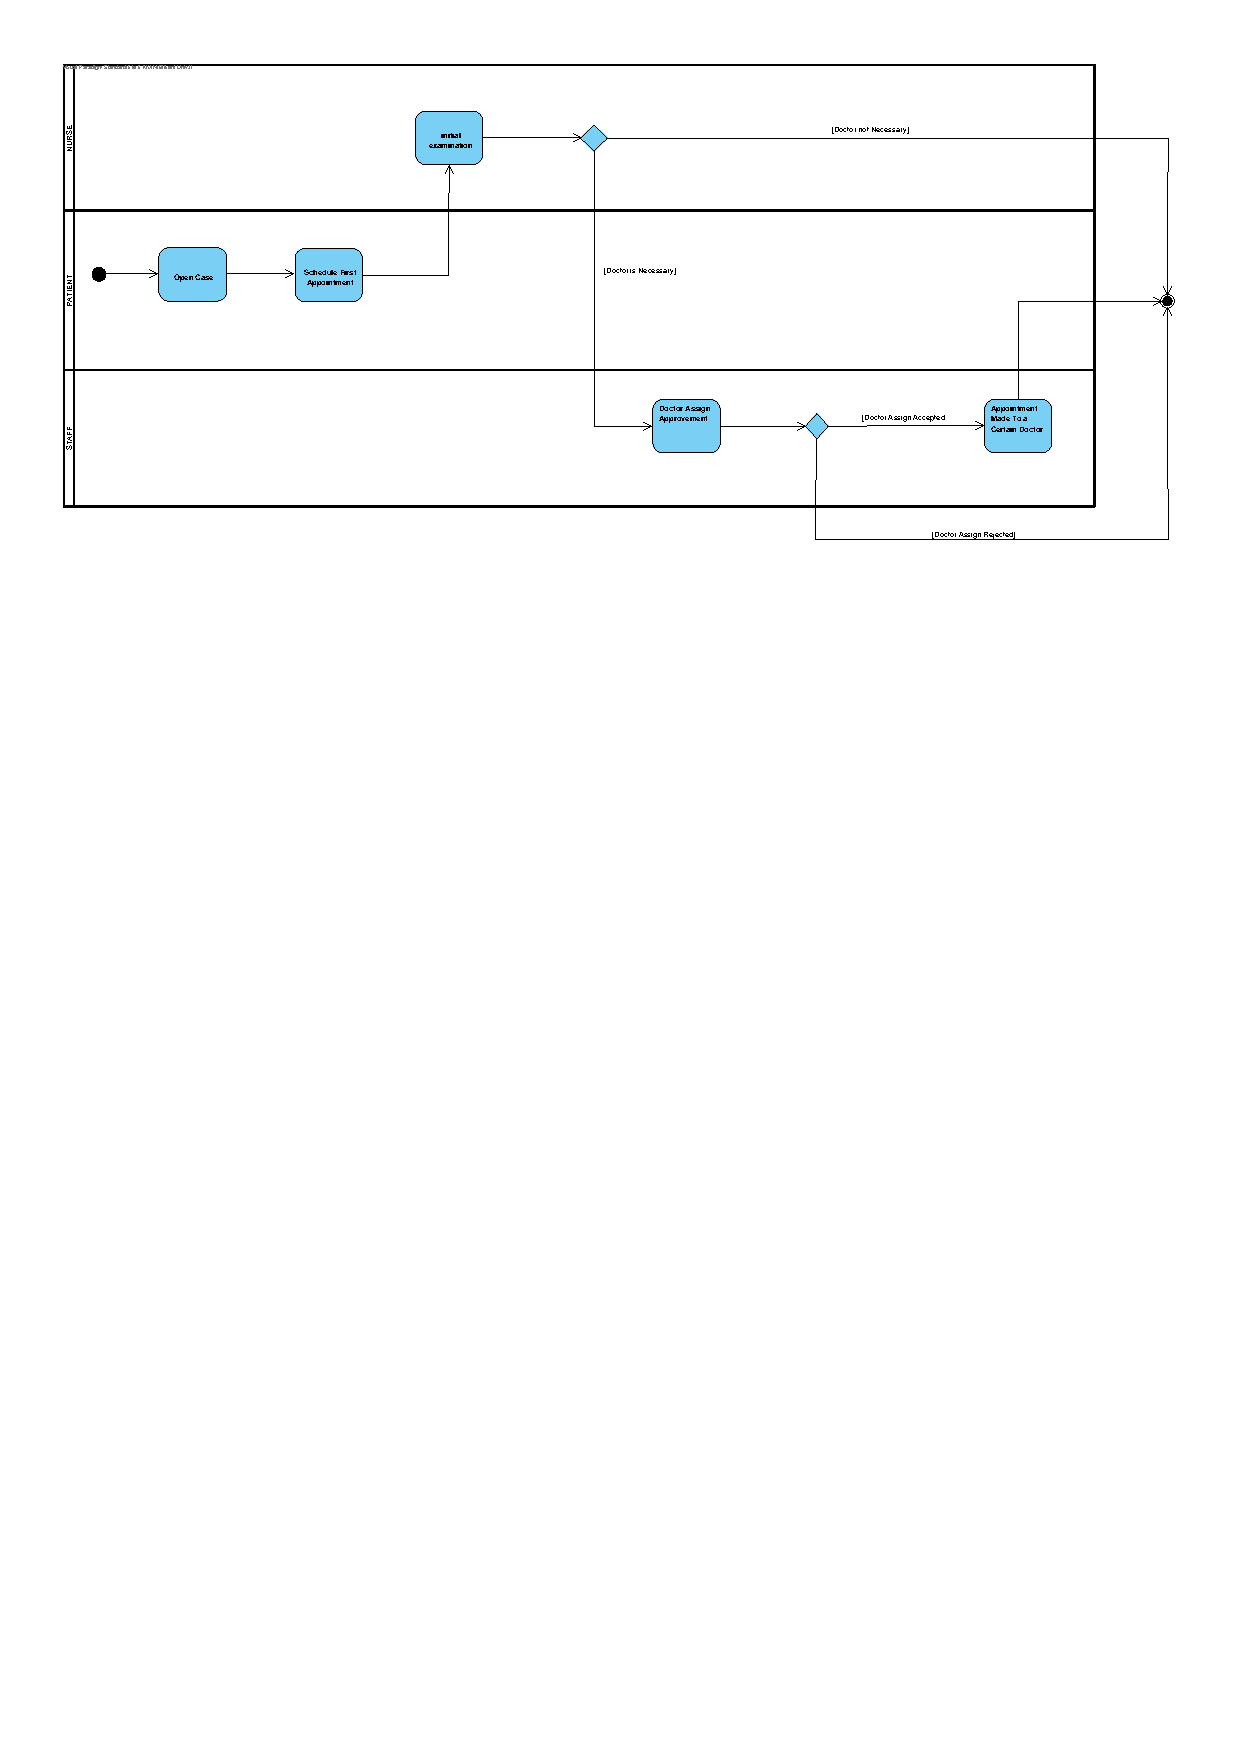
\includegraphics[width=\linewidth]{activity_diag_appointment}

  \subsubsection{State Diagram}

  The following diagrams demonstrates the various states a case can be in at a given time.

  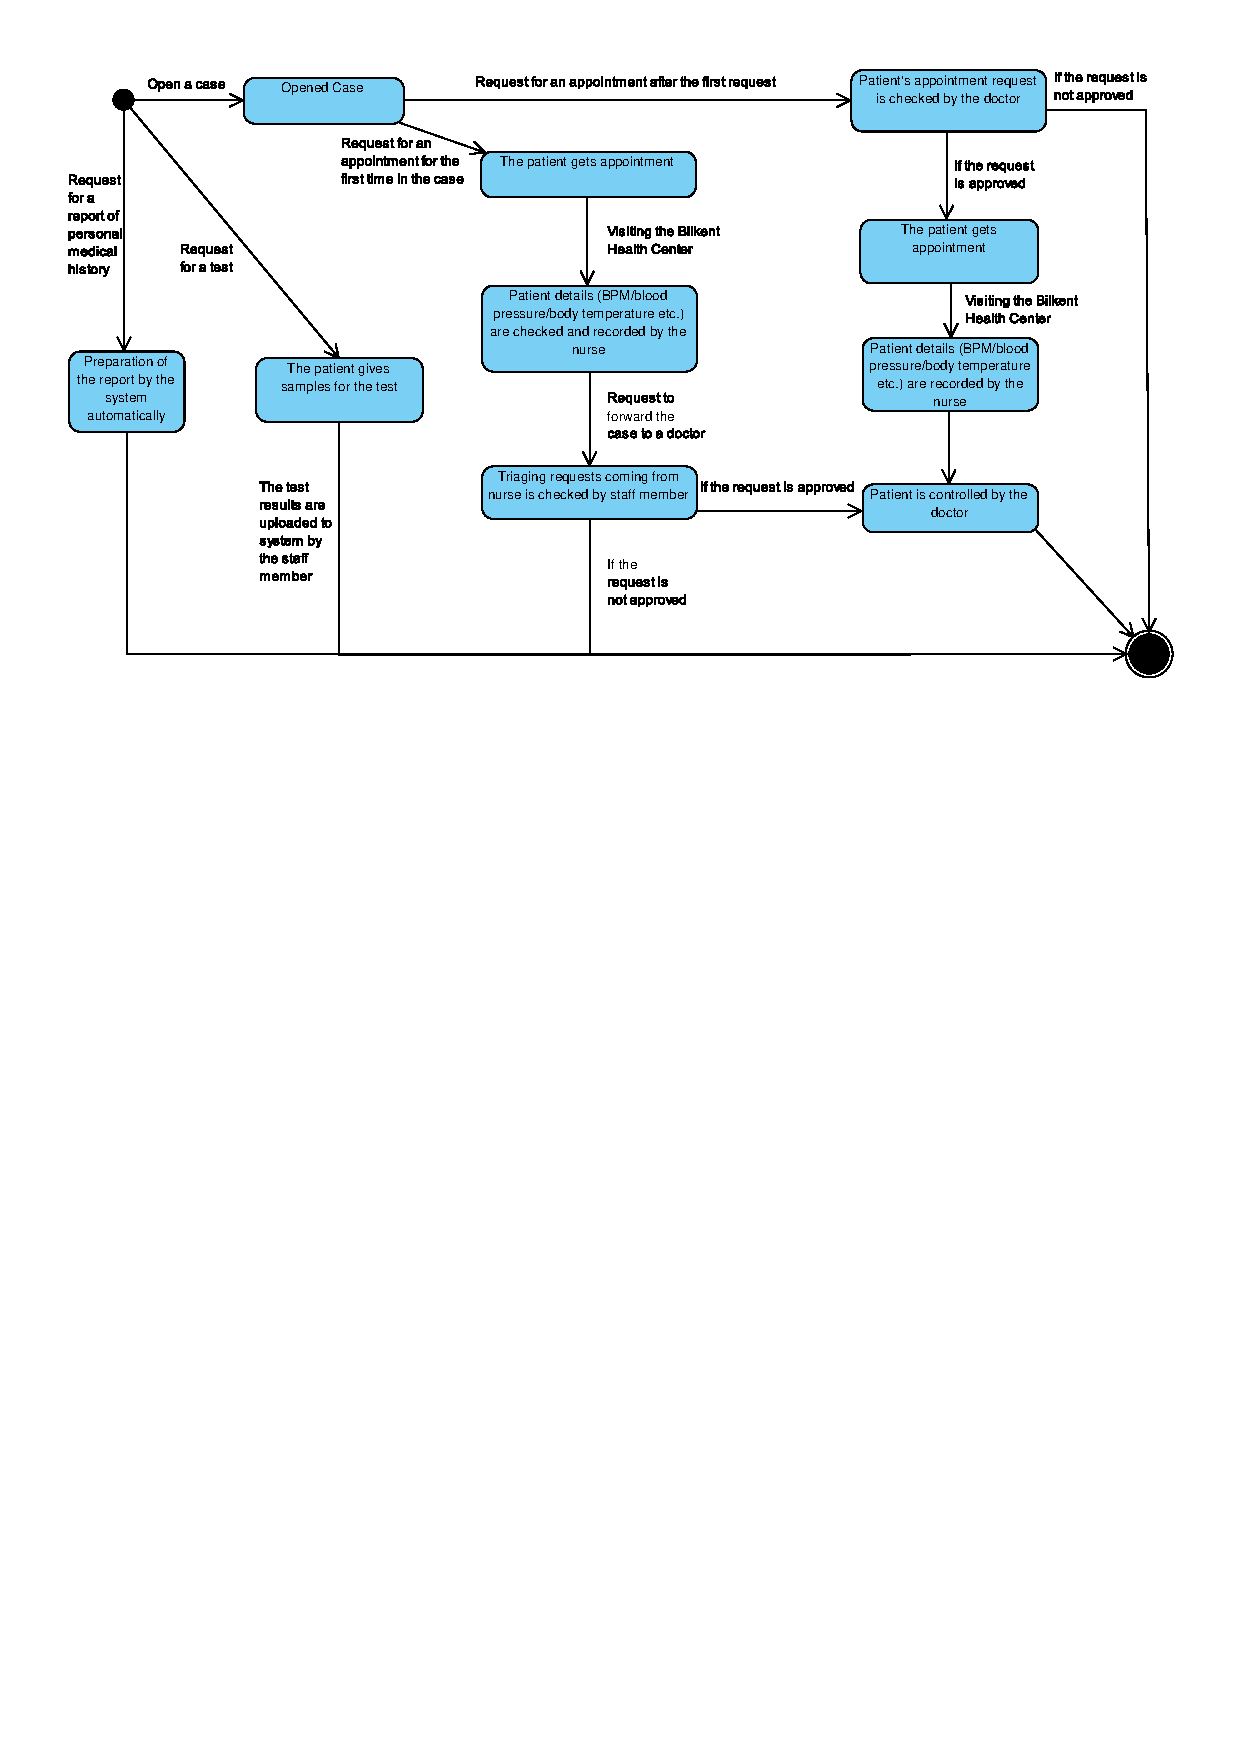
\includegraphics[width=\linewidth]{state_diag_patient.pdf}

  \pagebreak
  \subsubsection{Class Diagram}

  As our project is a web application, its structure follows the model/service/controller layer paradigm.
  The most consequential classes are services.

  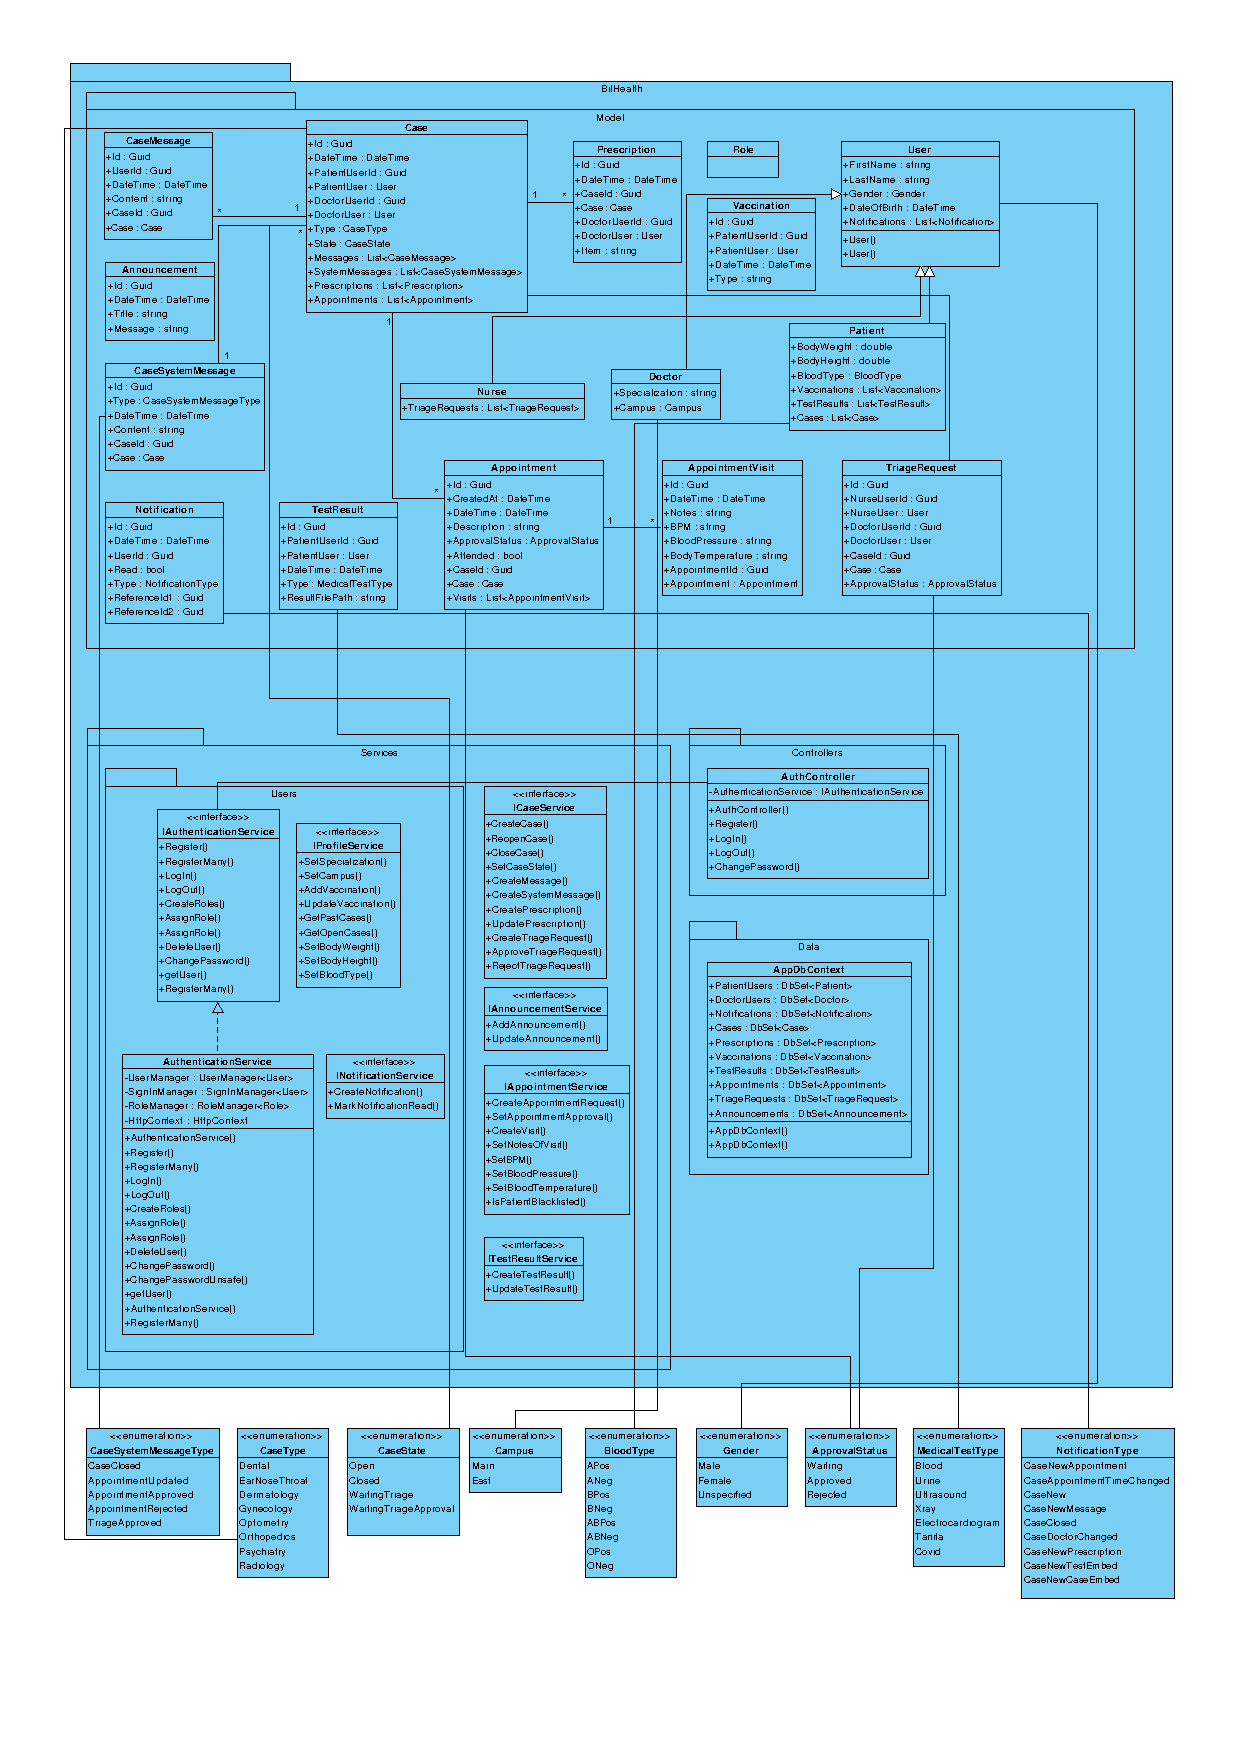
\includegraphics[width=\linewidth]{class_diag}

  \subsubsection{Sequence Diagram}

  The following diagram shows the rudimentary flow of method calls made during interactions with a case.

  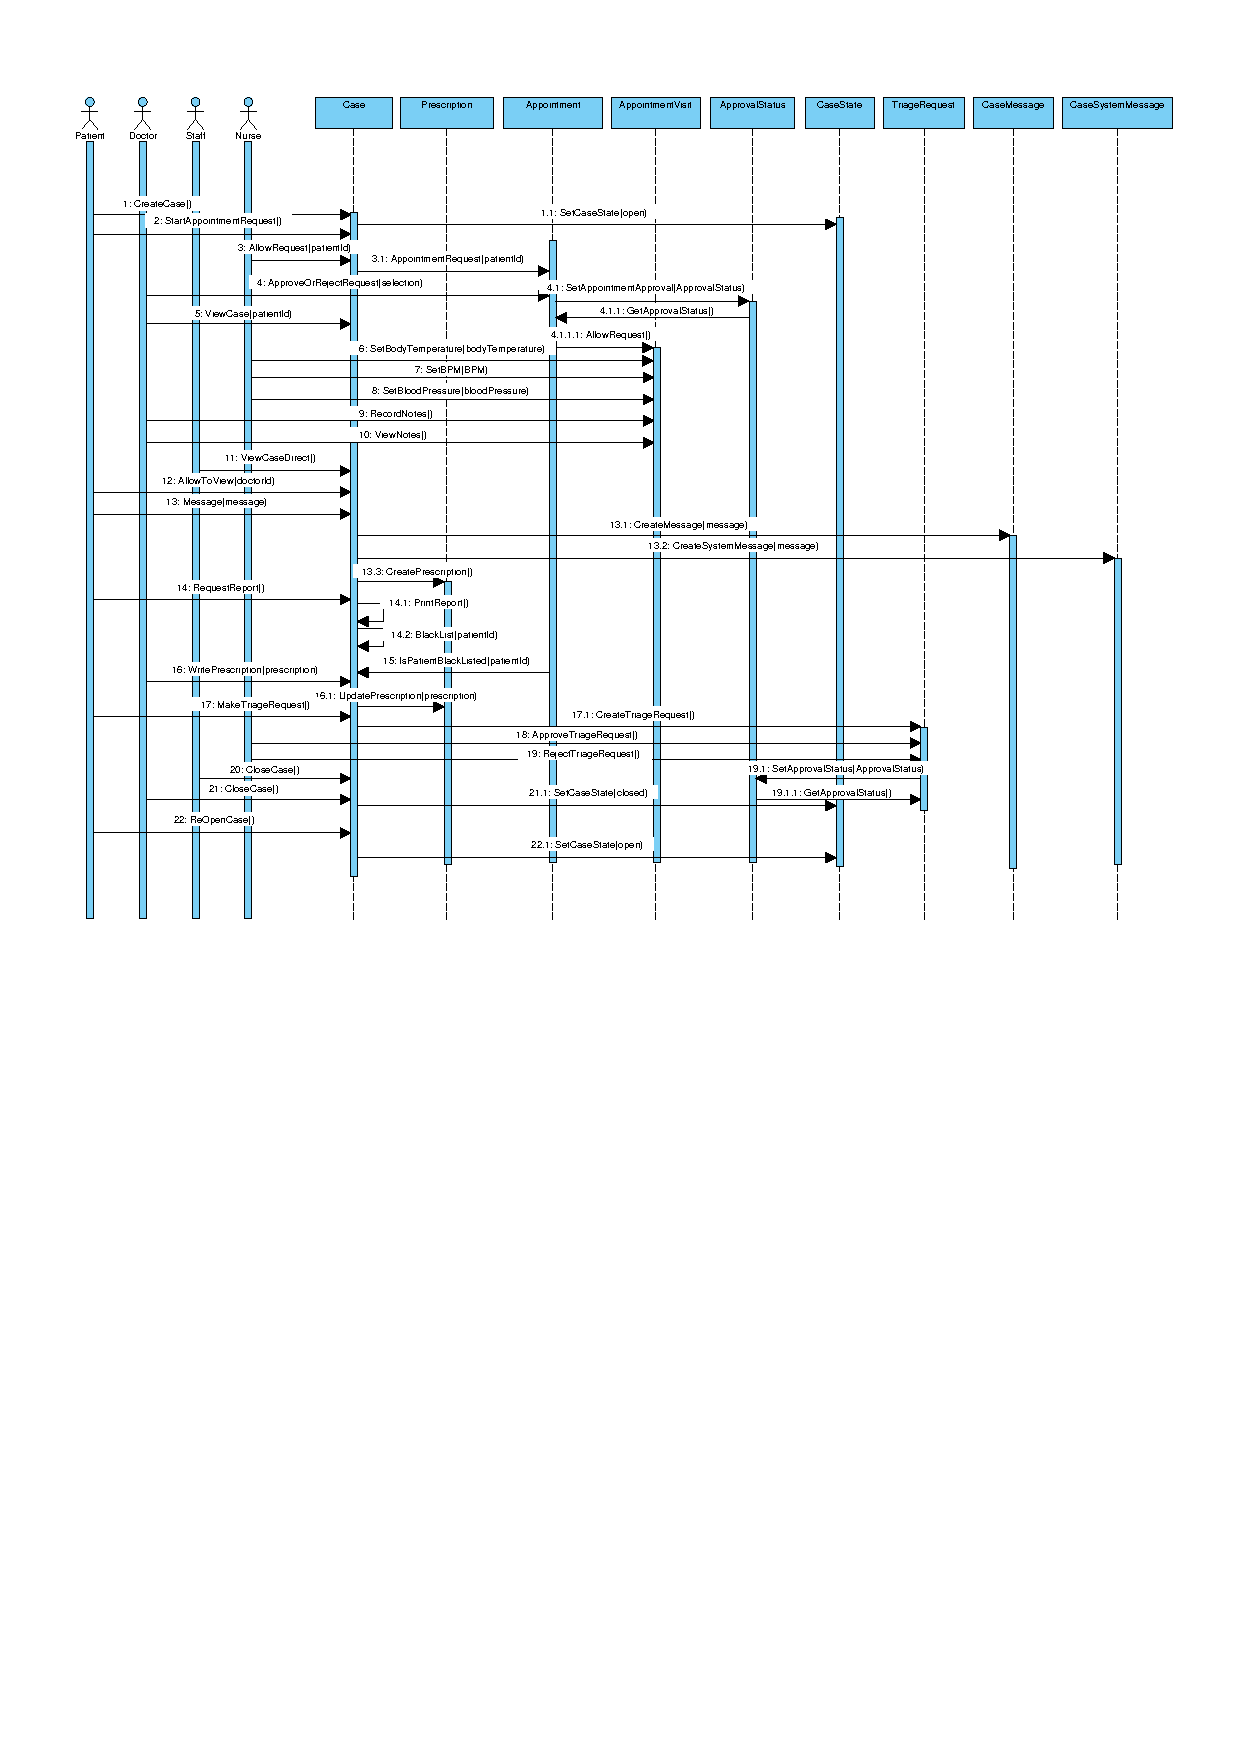
\includegraphics[width=\linewidth]{sequence_diag}

  \pagebreak
  \subsubsection{User Interface}

  The core \textit{case} functionality of our project bears a strong resemblence to that of GitHub's issue tracker.
  Of course, the format GitHub uses is not unique, but we think it is a good example nonetheless.
  Commits can be seen as appointment requests, visits, prescriptions, and such.
  Messages act as communication between the patient and the medical staff.
  System messages are used to alert users of any changes to the events.
  A sidebar can be used to display the case information.
  As such, our final user interface is likely to look similar to the following design.

  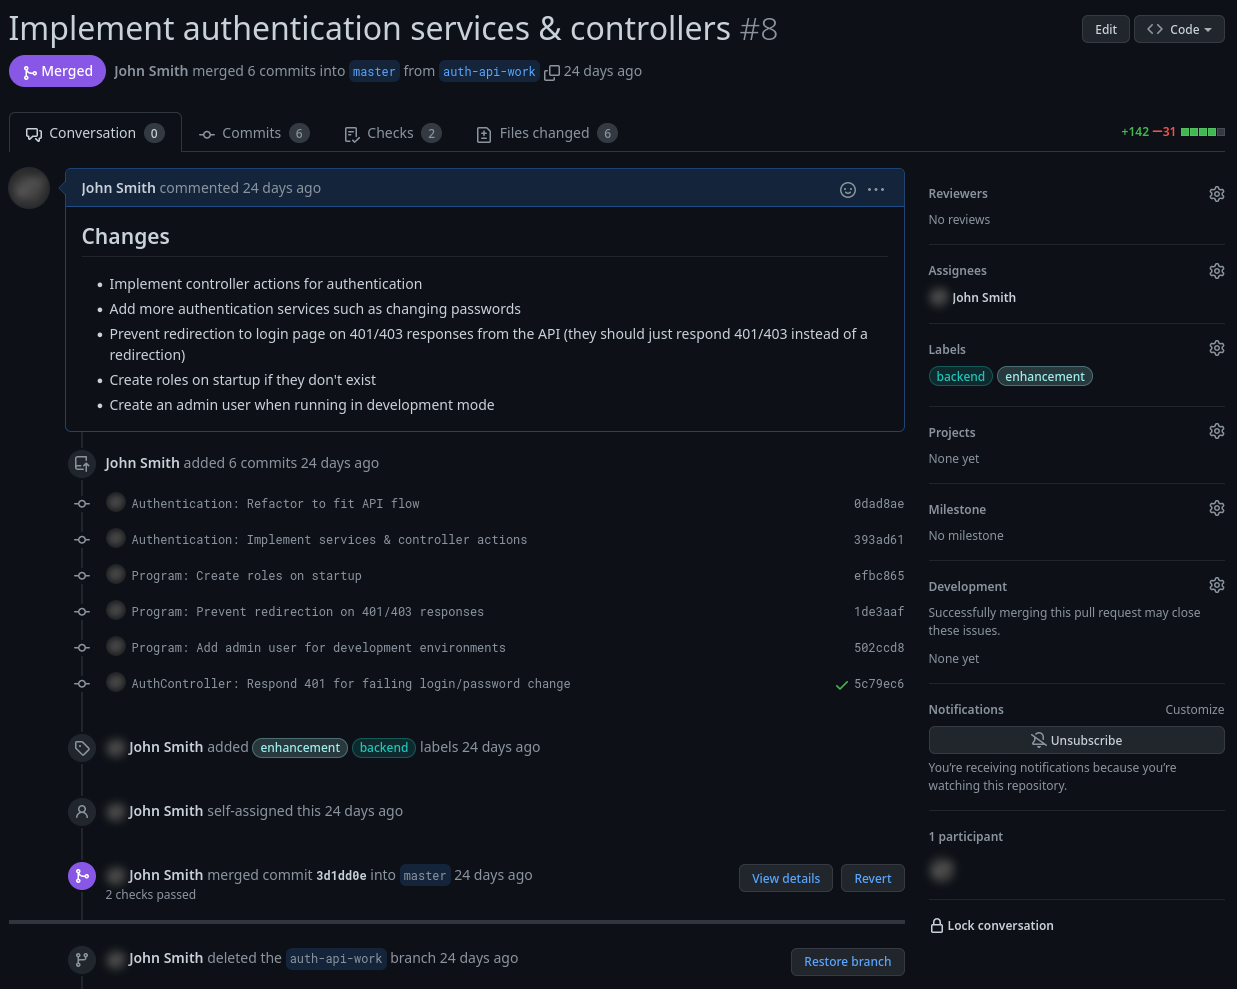
\includegraphics[width=\linewidth]{github_ui}

  \section{Glossary}

  \begin{itemize}
    \item \textbf{Case:} The main point of interaction between a patient and health center staff.
      A case contains all the relevant information on a particular medical situation,
      such as appointments and prescriptions.

  \end{itemize}

\end{document}
